\chapter{Propuesta y Detalles de Implementación}\label{chapter:proposal}

Al analizar los sistemas comparados en el capítulo anterior se nota la existencia
de grandes limitaciones expresivas para que el usuario exprese detalladamente las
características de su espacio de búsqueda. Por lo general, la solución de un problema de 
búsqueda se compone de una estrategia de búsqueda y un método de evaluación. 
Sin embargo, las implementaciones de estas soluciones necesitan además un mecanismo 
imperativo y poco descriptivo para generar muestras del espacio de búsqueda. 
Para hacer frente a estas limitaciones expresivas, el presente documento plantea le 
uso de un {\bf DSL} implementado para que el análisis de los problemas de búsqueda 
parta de una descripción expresiva y declarativa de su espacio de búsqueda.

Dicha herramienta fue desarrollada pensando en la comodidad del usuario a la hora de
describir y construir su espacio de interés. Por dicha razón, la biblioteca plantea
una filosofía constructiva, {\it “de abajo hacia arriba”} ({ \it “Bottom-Up”}), para la
construcción de dichas descripciones. La misma define una serie de patrones de diseño
con los que se puede expresar un espacio de búsqueda concreto con una clase de {\bf Python}, 
partiendo de los tipos básicos del lenguaje ({\it int}, {\it float}, {\it bool}, {\it str}).

Con dichos patrones el usuario puede describir la estructura y dimensión del espacio
relativo a la clase en cuestión, así como las características de cada uno de sus
componentes internos. Además, como el origen de la presente investigación se encuentra
en la imposibilidad de {\bf AutoGOAL} para describir dependencias contextuales, dichas pautas
fueron ideadas para que se pudieran expresar también dependencias y relaciones entre los
componentes internos de la clase en cuestión.

La sintaxis que propone el {\bf DSL} para describir los subdominios internos, en su mayoría,
son expresiones con estilo funcional y declarativo. La intención del autor era que,
en la medida de lo posible, las descripciones fueran lo más parecidas a las definiciones
de dominios matemáticos. En las definiciones matemáticas se suele expresar las características
de un conjunto a partir de las características singulares de un elemento cualquiera de este.
Un ejemplo simple del modelo al que se aspiraba es la siguiente definición de un subconjunto de
los números naturales:

\newcommand\Set[2]{\{\,#1\mid#2\,\}}
\newcommand\SET[2]{\Set{#1}{\text{#2}}}

\begin{align*}
    A := \Set{x \in \mathbb{N}}{x \ge 100, x \neq 101} \\
\end{align*}

Por otra parte, la propuesta de solución planteada, aporta sus propios mecanismos para la
generación de muestras de cada espacio en particular. Dichos mecanismos tienen como base la
generación de variables aleatorias y aunque la biblioteca cuenta con la implementación de
algunas de las distribuciones básicas, el usuario puede definir las suyas propias e incluso
redefinir las ya existentes. Asumiendo la existencia de dichas implementaciones, el resto del
proceso generativo se centra en la resolución de cada uno de los dominios concretos para cada
uno de los subespacios. Dichos dominios se encuentran expresados con la sintaxis del {\bf DSL}
y pueden contener dependencias entre ellos. Entre la lista de restricciones que el usuario puede
describir es importante resaltar dos de ellas, que suponen el mayor reto durante el proceso de
inferencia de los distintos dominios.

Las dependencias contextuales son un de los logros más importantes del presente trabajo. Para
su resolución, el mecanismo generativo necesita reconocer el orden topológico del grafo de
restricciones, para generar cada uno de los miembros en orden ascendente según el grado de
dependencia. Como a medida que se definen los distintos dominios dinámicos se van generando
muestras de los distintos subespacios, entonces el mecanismo generador necesita una última fase
en la que se revise la coherencia entre la muestra y las restricciones descritas.

El {\bf DSL} propuesto plantea también una sintaxis de restricciones definidas por funciones
externas, las cuales en muchos casos el mecanismo generativo las considera funciones
de ``{\it caja negra}''. En estos casos, al igual que sucede con las dependencias contextuales, es
necesario un análisis posterior al proceso generativo. Dicho análisis en esta ocasión es
mucho más propenso a errores, pues el mecanismo generativo no cuenta con información suficiente
para incluir a estas funciones en el proceso de inferencia y redefinición de cada dominio en
concreto. La filosofía {\it “prueba y error”} a la hora de generar muestras aleatorias es el
mecanismo más simple posible para crear elementos que cumplen con una cantidad finita de condiciones.
Aunque el autor ideó todos los protocolos que pudo para que la creación de muestras fuera lo más
lineal posible, para los casos de las funciones de ``{\it caja negra}'' lo más que se puede hacer es
optimizar el proceso de {\it “prueba y error”} aprendiendo de dichas equivocaciones.


\section{Descripción De La Biblioteca}\label{section:describe}

La interfaz pública de la biblioteca propuesta es la clase {\bf Domain} la cual es una factoría de espacios
aleatorios. En dicha clase, los tipos básicos y las funciones {\it lambdas} de {\bf Python} son todas
las herramientas necesarias para que los usuarios puedan definir sus clases, decorarlas describiendo
sus espacios búsqueda y posteriormente generar instancias de las mismas.


\begin{listing}[!ht]
    \begin{minted}{Python}
    from search_space import Domain
    ADomain = Domain[int]()
    a, _ = ADomain.get_sample()
    \end{minted}
    \caption{Generando un número entero}
    \label{lst:example}
\end{listing}

La sintaxis del ejemplo \ref{lst:example} es la mínima expresión del {\bf DSL} propuesto, donde basta con
definir el tipo del espacio de búsqueda para generar muestras dentro de la versión más extensa de dicho
espacio. Y aunque la herramienta se desarrolló con la intención de describir espacios más complejos,
como se puede ver en el ejemplo, se puede usar para generar muestras de los tipos básicos. Dicha
funcionalidad es la base sobre la que se sustenta el resto de funciones de la biblioteca.
Y como tal, el autor trabajó para que fueran lo más eficiente posible eficiente, aunque nunca serán
tan rápidos como los métodos nativos del lenguaje.

\begin{listing}[!ht]
    \begin{minted}{Python}
    from search_space import Domain
    ADomain = Domain[int] | (lambda x: (x >= 100, x != 101))
    a, _ = ADomain.get_sample()
    \end{minted}
    \caption{Generando un número entero con restricciones}
    \label{ex:func}
\end{listing}


En el ejemplo \ref{ex:func} se muestra uno de los mecanismos más importantes definido por el
    {\bf DSL}, la sintaxis para declarar restricciones. Con esta herramienta el usuario puede ser capaz de
expresar las dimensiones y características de sus espacios de interés. Como en los problemas de búsqueda el
costo temporal suele ser directamente proporcional a las magnitudes del espacio de búsqueda o a la estructura
del mismo entonces es de vital importancia poder describir los espacio de búsqueda de la forma más clara y
concreta posible. Una descripción detallada del espacio de búsqueda facilita en gran medida la comprensión
estructural del mismo y permite comenzar la búsqueda del elemento óptimo partiendo de un espacio inicial donde
la cantidad de elementos que no representan una soluciones factibles es mínima. El autor espera que se note las
similitudes entre esta sintaxis y las definiciones matemáticas, en concreto las restricciones de este ejemplo
con el subconjunto antes definido.

\subsection{Comparación con la sintaxis de AutoGOAL}

Como se ve en el ejemplo \ref{ex:class} la filosofía de la herramienta es que el usuario pueda “decorar” sus
clases declarando los distintos subespacios que la misma contiene. A partir de dicha implementación, basta
con replicar la sintaxis del primer o del segundo ejemplo, cambiar el tipo de {\bf Domain}, y las restricciones
en caso de ser necesario, para generar una instancia aleatoria del nuevo espacio descrito. Que la clase
    {\bf Domain} no solo soporte los tipos básicos sino que también pueda fabricar espacios de clases definidas por
los usuarios es la característica que hace que la propuesta de solución sea muy extensible y flexible. Las
descripciones del usuario puede ser tan anidadas como se necesite, mientras que las bases de la jerarquía
planteada en cada nivel estén definidas y debidamente descritas.

\begin{listing}[!ht]
    \begin{minted}{Python}
from search_space import Domain

class MySeachSpace:
    def __init__(
        self, 
        a: int = Domain[int](min = 10, max = 20),
        b: float = Domain[float] | (lambda x: (x != 0.5, x < 1)),
        c: str = Domain[str](options = ["SearchSpace", "Domain"])
    )
        self.a, self.b, self.c = a, b, c

MySeachSpaceDomain = Domain[MySeachSpace]()
my_seach_space_instance, _ = MySeachSpaceDomain.get_sample()
    \end{minted}
    \caption{Clase decorada para describir un espacio de búsqueda}
    \label{ex:class}
\end{listing}


La sintaxis elegida para la decoración de las clases se definió principalmente con la idea de
que los espacios sencillos se pudieran expresar de forma sencilla, y luego aquellos con estructuras más
complejas tuvieran descripciones expresivas pero no necesariamente sencillas.



\begin{listing}[!ht]
    \begin{minted}[autogobble]{Python}
from autogoal.grammar import ContinuousValue, CategoricalValue, DiscreteValue

class MySeachSpace:
    def __init__(
        self, 
        a: DiscreteValue(10, 20),
        b: ContinuousValue(0, 1),
        c: CategoricalValue("SearchSpace", "Domain")
    )
        if b in [0.5, 1]:
            raise ValueError('Invalid hyperparams')
        self.a, self.b, self.c = a, b, c
    \end{minted}
    \caption{Clase decorada con la sintaxis de AutoGOAL}
    \label{ex:autogoal}
\end{listing}


Haciendo referencia una vez
más a los orígenes de este trabajo, se puede comparar los ejemplos \ref{ex:autogoal} y \ref{ex:class} donde se
evidencia la diferencia entre una clase decorada con las herramientas de {\bf AutoGOAL} y otra con la propuesta
presentada. Nótese que efectivamente son espacios combinados pero extremadamente simples. En ambos casos las
modificaciones a lo que sería una clase de {\bf Python} común son mínimas. Nótese además que el {\bf DSL}
planteado es un tanto más verbosos que la sintaxis de {\bf AutoGOAL}; pero esto se debe a la propuesta de solución
aboga por una sintaxis coherente y consistente con el {\it “tipado estático”} de {\bf Python}, mientras que
    {\bf AutoGOAL} se apoya en las bondades del tipado dinámico.

\subsection{Flexibilidad de la Función de Restricciones, Dependencias Contextuales y Espacios Tensoriales}

Como se comentó anteriormente, dos de los aportes más importante de la propuesta son las dependencias
contextuales y las descripciones de {\it “caja negra”}. Ambas funcionalidades son alteraciones de la sintaxis
antes expuesta para expresar las restricciones de un dominio específico.

\begin{listing}[!ht]
    \begin{minted}{Python}
class MySeachSpace:
    ADomain = Domain[int](min = 10, max = 20)
    def __init__(
        self, 
        a: int = ADomain,
        b: float = Domain[float] | (
            lambda x, y = ADomain: (x < y)
        )
    )
        self.a, self.b = a, b

    \end{minted}
    \caption{Clase que describe un espacio dependedientes del contexto}
    \label{ex:classDep}
\end{listing}


En el ejemplo \ref{ex:classDep} se muestra
uno de los casos más clásicos de dependencias contextuales, el espacio aleatorio de dos números donde el
primero es mayor que el segundo. En dicho ejemplo se escribe la función de restricciones como una función
de dos parámetros donde el primero es un elemento cualquiera del espacio en cuestión y el segundo es un
elemento cualquiera de una definición previa. Dado estos dos elementos cualesquiera, el usuario puede
describir una relación entre ambos espacios a partir de la relación existente entre dos de sus elementos.

\begin{align*}
    A := \Set{(x, y) \in \mathbb{N} \times \mathbb{N}}{x < y} \\
\end{align*}

Es probable que el lector, al analizar el caso de estudio seleccionado para mostrar la sintaxis de dependencias
contextuales, piense en que dicho problema se describe mejor con la definición matemática anterior que con la
clase del ejemplo \ref{ex:classDep}. Y es que la intención de dicho ejemplo era únicamente introducir la sintaxis para la decoración
de las clases con espacios sensibles al contexto. El {\bf DSL} cuenta su propia sintaxis para definir espacios de más
de una dimensión, como sería el caso del dominio planteado en la definición matemática anterior. Dicha sintaxis
no solo se limita a dimensiones predefinidas, ni a restricciones de índices fijos como es el caso del dominio relativo
al parámetro {\bf a} de la clase del ejemplo 6, que intenta simular la definición teórica del problema planteado como ejemplo.
Sino que, como se aprecia en el dominio relativo al parámetro {\bf b} de la misma clase, la sintaxis definida para los espacios
multidimensionales es capaz de describir dominios donde el tamaño de las dimensiones está descrito por otro espacio
aleatorio y las restricciones se les aplican secuencialmente a cada subelemento de dicho espacio.


\begin{listing}[!ht]
    \begin{minted}{Python}
class MySeachSpace:
    ADomain = Domain[int](min = 10, max = 20)
    def __init__(
        self, 
        # Espacio de todas las tuplas de dos elementos,
        # tal que el primer elemento es menor que el segundo
        # (10, 100) pertenece al espacio
        # (0, 0) y (1, 0) no pertenecen
        a: int = Domain[int][2] | (
            lambda x: (x[0] <  x[1])
        ),
        # Espacio todas las matrices cuadradas, 
        # tal que todos los valores internos son menores 
        # sus dimensiones 
        # [0] pertenece, pero la siguiente matriz no 
        # [[1,0]]  
        # [[1,2]]
        b: float = Domain[float][ADomain][ADomain] | (
            lambda x, i, j, y = ADomain: (
                x[i][j] < y
            )
        )
    ):
        self.a, self.b = a, b

    \end{minted}
    \caption{Clase que describe un espacio de búsqueda compuesto por listas de distintas dimensiones }
    \label{ex:classList}
\end{listing}

Nótese que, en el ejemplo \ref{ex:classList} se evidencia la flexibilidad de la sintaxis para definirle restricciones a un
nuevo dominio. El número de variables de entrada del delegado de restricciones puede crecer según las necesidades
del usuario; siendo siempre mayor que uno, pues la primera variable siempre hace referencia a un elemento cualquier
del dominio en cuestión. Salvo dicho primer elemento, todas las variables de la función de restricciones a las que
el usuario no le asigne un dominio externo harán referencia a índices dinámicos que apuntan a cada una de las
dimensiones del espacio en cuestión de forma ascendente. Por ejemplo, en la definición del parámetro {\bf b} del
ejemplo anterior las variables {\bf x}, {\bf i}, {\bf j}, y {\bf y} hacen referencia a un elemento cualquiera
dominio de en cuestión, al índice dinámico de la primera dimensión de los elementos de dicho conjunto, al índice dinámico
de la segunda dimensión de dichos elementos y a un elemento cualquiera del conjunto {\bf ADomain}.

\subsection{Restricciones Imperativas}

El caso de las restricciones de {\it “caja negra”} se ejemplifica con el ejemplo \ref{ex:classFunc}. Con esta funcionalidad
la biblioteca le deja la puerta abierta al usuario para que pueda describir su dominio de forma imperativa.
Como se puede ver en el ejemplo; solo es necesario decorar una función de {\bf Python} donde se describa un
procesamiento sobre los parámetros de entrada, para que el usuario pueda incluir la llamada a esta dentro de
la lista de restricciones. El {\bf DSL} incluirá las llamadas a dicha función dentro de su mecanismo generativo.
Luego de que culmine el cómputo de la misma, dicho mecanismo utilizará sus resultados para realizar el resto
de operaciones que fueron descritas en la lista de restricciones.

\begin{listing}[!ht]
    \begin{minted}{Python}
from search_space import FunctionalConstraint
@FunctionalConstraint
def IsEven(x):
    for i in range(2, x/2):
        if x % i == 0:
            return False
        
    return True

@FunctionalConstraint
def Factorial(x):
    resutl = 1
    for i in range(2, x + 1):
        resutl *= i
    return resutl

class MySeachSpace:
    ADomain = Domain[int] | (lambda x: IsEven(x)))
    def __init__(
        self, 
        a: int = ADomain,
        b: float = Domain[float] | (
            lambda x, y = ADomain: (x < Factorial(y))
        )
    )
        self.a, self.b = a, b

    \end{minted}
    \caption{Espacio de búsqueda con restricciones imperativas}
    \label{ex:classFunc}
\end{listing}


Que la ejecución de estas funciones de {\it “caja negra”} se realicen antes o después del proceso de
inferencia y redefinición de los distintos dominios dinámicos en cuestión depende únicamente de los
parámetros con los que el usuario llame a dicha función dentro de la lista de restricciones. El resultado
de esta función se tendrá en cuenta para la redefinición del dominio en cuestión siempre que sus parámetros
no hagan referencia al dueño de dicho dominio. Por tanto, una función de ``{\it caja negra}'' no puede modificar
el dominio de una variable aleatoria de la que depende su resultado. En cualquier otro caso, las funciones de
    {\it “caja negra”} y todas sus dependencias se resuelven previo a la redefinición del dominio en cuestión. Bajo
la descripción anterior se puede interpretar que el resultado de la función {\it Factorial} si participa en el
proceso de reducción e inferencia, mientras que la función {\it IsEven} no lo hace.

\subsection{Restricciones Condicionales}

Para terminar con la descripción de la sintaxis del {\bf DSL} propuesto y siendo consecuente con la comparación realizada
en el estado del arte, luego de haber expuesto tanto su mecanismo para describir dependencias contextuales, como su
habilidad para expresar espacios de dimensiones dinámicas, véase en el ejemplo \ref{ex:classCond} la sintaxis propuestas para
expresar descripciones de espacios con restricciones condicionales. El {\bf DSL} no aporta ninguna estructura de control
de flujo para describir estas restricciones condicionales, este anima al usuario a plantear dichas restricciones
haciendo uso de operadores lógicos. Dichos operadores presentan una implementación de corte, ósea si es suficiente
con el resultado del operador de la izquierda para determinar el resultado final de la operación entonces el operador
de la derecha nunca será computado. El autor considera dicha propuesta como la opción más expresiva analizada; aunque
lo ideal sería poder incluir estructura de control de flujo al estilo de la compresión de listas  ({\it “list comprehension”})
de {\bf Python}, lamentablemente la flexibilidad de dicho lenguaje no alcanza tal punto.

\begin{listing}[!ht]
    \begin{minted}{Python}
from search_space import FunctionalConstraint

class MySeachSpace:
    ADomain = Domain[int](max = 100)
    def __init__(
        self, 
        a: int = Domain[int] | (
            # Si y es un número => espacios de los enteros
            # Si y no es un número => espacio que solo contiene
            # al número 10
            lambda x, y = ADomain: (IsEven(y) | x == 10 )
        ),
        b: float Domain[float] | (
            # Si y es un número => espacios de los enteros
            # Si y no es un número => espacio de los reales 
            lambda x, y = ADomain: (IsEven(y) & x % 1 == 0 )
        )             
    ):
        self.a, self.b = a, b

    \end{minted}
    \caption{Espacio de búsqueda con restricciones condicionales}
    \label{ex:classCond}
\end{listing}

\subsection{Generación de Muestras}

Como se ha comentado con anterioridad la propuesta de solución debe plantear dos mecanismos, uno para describir espacios
de búsquedas y otro para generar muestras de lo previamente descrito. Hasta el momento se ha hecho énfasis en el componente
descriptivo y a lo largo de toda las explicaciones anteriores se ha hecho referencia a distintos procesos del componente generativo.

Dicho componente, desde sus inicios, se desarrolló con la intención de alejarse lo más posible de las filosofías de
    {\it “prueba y error”}. Este, partiendo de la base de un espacio de búsqueda descrito con las herramientas anteriormente
detalladas, modela todas las descripciones como una jerarquía de clases sobre la cual pueda detectar las distintas
relaciones entre los espacios descritos, reconocer el orden topológico de dichas descripciones y preparar todas las
herramientas necesarias para construir las respectivas muestras. En el momento que una instancia de la
clase {\bf Domain} llama al método {\it get\_sample} el mecanismo generativo, apoyado en la jerarquía antes descrita, comienza
a construir la nueva muestra.
% en orden topológico y con la misma filosofía de las descripciones {\it “de abajo hacia arriba”}.

Como se explicó anteriormente todo el proceso generativo está sustentado por la generación de variables aleatorias
con una cierta distribución. Sin embargo, los procesos realmente aleatorios dentro de la creación de muestras son la
selección de opciones, como es el caso de los tipos básicos {\it string} y {\it bool}, y la generación numérica, para los {\it int} y los
{\it float}. El resto de los mecanismos se limitan en crear las instancias de los tipos adecuados con los parámetros correctos. Para que
la generación sea un proceso lineal el componente generativo trasmite cada una de las restricciones descritas en los niveles
superiores de la jerarquía descrita hacia los niveles inferiores donde se encuentran los tipos básicos antes mencionados.
Con la interpretación de estas restricciones la biblioteca le puede asignar a cada uno de los tipos básicos el dominio más
amplio que cumpla con todas las condiciones para que el resultado del proceso aleatorio sea consecuente y efectivo.

La coherencia y consistencia de las muestras con sus respectivas descripciones es uno de los temas más importantes de los que
se debe encargar el componente generativo, sobre todo con la presencia de dependencias contextuales o restricciones de
``caja negra''. Por ejemplo, véase en el ejemplo \ref{ex:classList} la descripción del dominio del parámetro {\bf b}, en este se describe una matriz cuadrada
donde no solo se igualan las dimensiones de la misma con el espacio aleatorio {\bf ADomain} sino que además se señala que todo
valor en la matriz es menor que dichas dimensiones. Como se puede apreciar es necesario que el proceso generativo sea coherente
y robusto con las muestras del dominio {\bf ADomain}, pues para un mismo proceso constructivo el valor aleatorio de dicho dominio
debe ser el mismo tanto para las dimensiones de la matriz como para el límite de los valores de la misma.

Con respecto a las dependencias contextuales, como se ha mencionado en diversas ocasiones, que la generación de muestras se realiza
en orden topológico; por lo que al momento de generar muestras de un subcomponente específico ya se ha
generado las muestras de las que depende dichos subcomponentes. Del razonamiento anterior se deriva que al momento de generar
un valor aleatorio para cualquiera de los tipos básicos dentro del su dominio dinámicamente inferido ya se encuentran resueltas
las restricciones contextuales.

Por otra parte, como ya se mencionó con anterioridad, la transición de las restricciones de “{\it caja negra}” a través de
toda la jerarquía que describe el espacio de búsqueda del usuario depende únicamente de los parámetros con los que
dicho usuario utilice la función, Véase en este caso las restricciones del ejemplo \ref{ex:classFunc}, donde se definen dos nuevas
restricciones {\bf IsEven} y {\bf Factorial}. Dichas definiciones se diferencia únicamente por sus nombres y sus procesos internos,
pero para el componente generativo de la propuesta de solución son dos funciones que esperan un valor de entrada y
retornan otro de salida.

Sin embargo, durante el proceso constructivo la muestra para el parámetro {\bf b} se genera de forma lineal, mientras que la
muestra del parámetro {\bf a} depende del mecanismo de “{\it prueba y error}”. Esto se debe a que el parámetro con el que se llama
a la función {\bf IsEven} representa un elemento cualquiera del dominio del parámetro {\bf a}, por lo tanto la validez de cualquier
posible muestra depende del resultado de dicha función evaluada en dicha muestra. Por otra parte, el caso de las
restricciones aplicadas al dominio del parámetro {\bf b} hacen referencia a una comparación con respecto al resultado de una
función que depende de un parámetro sensible al contexto que puede ser resuelto previo a la generación de la muestra en
cuestión, como se explicó anteriormente.

Para optimizar los casos donde la única opción es la “{\it prueba y error}” la biblioteca cuenta con un mecanismo para “aprender”
de cada error. Dicho mecanismo solo esta disponible para los errores en la generación de muestras de tipos básicos, pues el
resto son espacios combinatorios donde descartar opciones no es trivial. En los tipos simples, por otro lado, descartar un
elemento no es más que una nueva delimitación del dominio dinámico y contextual.

\section{Ideas e Implementación}


Luego del análisis realizado al estado del arte en el que se desarrollaría la investigación, la implementación de
la propuesta de solución se realizó entendiendo que la herramienta final no solo debía resolver dos problemas
(expresividad y generación) sino que además debía ser un sistema con dos componentes independientes capaces de
operar juntos. Como se comentó anteriormente, dichas dos piezas por lo general se explotarán en momentos distintos
del programa del usuario, las descripciones deberían interpretarse una única vez, mientras que el sistema generador
debe poder ser ejecutado tanto como el usuario lo requiera. Debido a lo anterior, a lo largo del desarrollo de la
herramienta frente a todo problema el autor siempre analizó si la solución del mismo podía ser computada total o
parcialmente al momento de interpretar cada descripción y únicamente en caso contrario dicho problema se resuelve desde
cero al momento de generar muestras.


Además de en la filosofía anteriormente descrita, el desarrollo se apoyó en otra serie de consideraciones.
Primero, siempre se consideró más importante la velocidad de generación que la memoria de ejecución, siendo 
consecuentes con la filosofía básica del desarrollo, si la información puede ser computada en tiempo de compilación y
posteriormente utilizada para simplificar el proceso de generación se debe almacenar la misma. Segundo, con el objetivo
fijado en las descripciones de dependencias contextuales, se consideró que dicho problema es naturalmente recursivo, por
lo que los procesos de compilación e interpretación de las descripciones y la generación de muestras deberían tener
dicha naturaleza.

Luego, siendo conscientes de los posibles usos de la herramienta (generación con dominio sin restricciones, con
restricciones deterministas o con restricciones contextuales), se analizó que existirían procesos innecesarios
para casos concretos, por lo que se desarrolló toda la infraestructura necesaria para comprender el caso de uso
especificado por el usuario y crear únicamente las clases y herramientas imprescindibles. Por último, como la
propuesta de solución es un {\bf DSL} para la descripción y delimitación de los dominios de interés de los usuarios,
todos los algoritmos y teorías sobre la compilación e interpretación de lenguajes serían una sólida base desde
donde partir para la búsqueda de soluciones, así como la lógica matemática y la teoría de conjunto sería una
fuente de inspiración para la sintaxis y las funcionalidades del sistema.

El centro toda la lógica de la biblioteca es la clase {\bf BasicSearchSpace}. La misma cuenta con una
serie de métodos e implementaciones que se detallarán a lo largo del capítulo. Dicha clase cuenta además con
sus propios ``{\it métodos mágicos}'' para que toda clase que herede de esta pueda ajustar los procesos antes comentados
a su dominio y funcionalidad específica.


\subsection{Interfaz Domian, Factoría de Espacios de Búsqueda}

Como ya se ha explicado anteriormente, la herramienta pública de la biblioteca es la clase {\bf Domian}. Esta es una
factoría de clases que heredan de la clase \newline {\bf BasicSearchSpace}. La biblioteca cuenta con 10 de estas clases, una
por cada tipo básico ({\it int}, {\it float}, {\it str}, {\it bool}), dos para las estructuras como listas y clases,
otras tres que representan los operadores de tipo ({\it Union}, {\it Self}, {\it Optional}) y una última para los
espacios con dependencias contextuales. Dicha factoría crea la instancia relativa al tipo estático correspondiente que el usuario
especifique con la sintaxis vista en secciones anteriores. Dicha instancia no será creada hasta que la clase
    {\bf Domian} ejecute su método {\it \_\_call\_\_} o su método {\it \_\_or\_\_}, dejando espacio para que el usuario
luego de especificar el tipo pueda continuar determinando las dimensiones del espacio que quiere describir.
\newline

% Define block styles
\tikzstyle{decision} = [diamond, draw, text centered, minimum height=2em, text width=8em]


\tikzstyle{block} = [rectangle, draw, text centered, rounded corners, minimum height=4em, text width=10em]
\tikzstyle{line} = [draw, -latex']
\tikzstyle{cloud} = [draw, ellipse, minimum height=2em, text width=8em]

% \begin{tikzpicture}[node distance = 2cm, auto]
%     % Place nodes
%     \node [block] (init) {datos iniciales};
%     \node [decision, below of=init] (has_options) { ?` el parámetro {\bf options} es distrinto de {\bf None} ?  }
%     \node [block, left of=has_options] (categorical) { clase = espacio de búsqueda categorical };
%     \node [block, right of=has_options] (natural) { class = espacio de búsqueda relativo al tipo };
%     % \node [cloud, right of=init] (system) {system};
%     % \node [block, below of=init] (identify) {identify candidate models};
%     % \node [block, below of=identify] (evaluate) {evaluate candidate models};
%     % \node [block, left of=evaluate, node distance=3cm] (update) {update model};
%     % \node [decision, below of=evaluate] (decide) {is best candidate better?};
%     % \node [block, below of=decide, node distance=3cm] (stop) {stop};
%     % Draw edges
%     \path [line] (init) -- (has_options);
%     \path [line] (has_options) -| node [near start] {si} (categorical);
%     \path [line] (has_options) -| node {no} (natural);

%     % \path [line] (update) |- (identify);
%     % \path [line] (decide) -- node {no}(stop);
%     % \path [line,dashed] (expert) -- (init);
%     % \path [line,dashed] (system) -- (init);
%     % \path [line,dashed] (system) |- (evaluate);
% \end{tikzpicture}

\begin{tikzpicture}[node distance = 2cm, auto][!ht]

    % Place nodes
    \node [block] (init) {Tipo, dimensiones, parámetros y lista de restricciones};
    \node [cloud, right= 2.5cm of init, text width=12em] (hasOptions) { ?`El parámetro {\bf options} es distinto de {\bf None}?};
    \node [block, below= 1.2cm of hasOptions] (categorical) {clase = espacio de búsqueda categórico};
    \node [block, below= 1.2cm of init] (normal) {clase = espacio de búsqueda relativo al tipo estático};
    \node [cloud, below= 1.2cm of normal] (dim) { ?`Es un espacio multidimensional?};
    \node [block, right= 3.7cm of dim] (tensor) {clase = espacio tensorial de tipo igual a la clase previa};
    \node [cloud, below= 1.2cm of dim] (restricciones) { ?`Hay restricciones contextuales?};
    \node [block, right= 3.7cm of restricciones] (ss) {clase = espacio sensible al contexto de tipo igual a la clase previa};
    \node [block, below= 1.1cm of restricciones] (stop) {Generación de una nueva instancia de la {\bf clase} correspondiente};

    % Draw edges
    \path [line] (init) -- (hasOptions);
    \path [line] (hasOptions) -- node {si} (categorical);
    \path [line] (hasOptions) -- node {no} (normal);
    \path [line] (categorical) -- (dim);
    \path [line] (normal) -- (dim);
    \path [line] (dim) -- node {si} (tensor);
    \path [line] (dim) -- node {no} (restricciones);
    \path [line] (tensor) -- (restricciones);
    \path [line] (restricciones) -- node {si} (ss);
    \path [line] (ss) -- (stop);
    \path [line] (restricciones) -- node {no} (stop);


\end{tikzpicture}
\newline

Una vez fijado el tipo y las dimensiones, el usuario deberá utilizar la sintaxis de {\bf Python} para llamar a una función
o asignarle una lista de restricciones al dominio mediante el operador ``|'', sintaxis vista en la secciones \ref{section:describe}.
Cualquiera sea la elección del usuario, la clase  {\bf Domian}  creará la nueva instancia del espacio de
búsqueda correspondiente, en dependencia del tipo, las dimensiones, los parámetros iniciales provistos al constructor
de la clase  {\bf Domian}  y el hecho de que se le defina restricciones al espacio o no. La lógica implementada para seleccionar
la clase heredera correspondiente se muestra en la imagen siguiente mediante un diagrama de flujo. Dicho mecanismo fue
implementado para que el espacio creado sea aquel que contenga las herramientas mínimas para generar muestras del
espacio descrito.
% \newline
% \newline





\subsection{Interpretación de las Funciones de Restricción}

Una vez determinado el tipo específico asociado al espacio de búsqueda que el usuario intenta describir comienza
el proceso de interpretación y almacenamiento de las distintas restricciones. Como se vio en secciones
anteriores, las restricciones se describen mediante la sintaxis de expresiones lambdas de {\bf Python}, lo que
significa que dichas restricciones no son más que una función anónima del lenguaje. En este caso específico
se puede señalar que las restricciones son funciones que en gran medida dependen de sus parámetros de entrada.

Para obtener toda la información descrita por el usuario dentro de dichas funciones, la biblioteca cuenta con
una jerarquía de clases con la que se pueden representar los {\bf ASTs} de cada una de las cadenas del lenguaje definido
por el {\bf DSL} para la descripción de restricciones. Cada una de las clases que componen dicha jerarquía cuenta con
la implementación de los ``{\it métodos mágicos}'' de las operaciones permitidas por la gramática para cada nodo en particular. De esta manera,
si se usa como entrada para una función de restricciones instancias de clases específicas de dicha jerarquía,
entonces de ser correcta la descripción implementada el resultado de dicha función sería el {\bf AST} de las restricciones
descritas, de lo contrario se producirá un error de sintaxis. En la figura \ref{chap2:grammar} se puede ver la gramática que se 
definió para dichas descripciones, a partir de la cual se implementó dicha jerarquía.



\setlength\LTleft{0cm}
\begin{longtable}{  c  }
    \caption{Gramática de Restricciones}\label{chap2:grammar}                                                                    \\
    \endfirsthead
    % \multicolumn{1}{c}{\tablename\ \thetable\ -- \textit{Continued from previous page}} \\
    \hline
    \endhead
    \hline
    % \multicolumn{1}{r}{\tablename\ \thetable\ -- \textit{Continued on next page}}       \\
    \endfoot
    \hline
    \endlastfoot

    $\hspace{-2.5cm} \bnfpn{Constraint} \bnfpo \bnfpn{Constraint} \bnfsp | \bnfsp \bnfpn{Constraint}$                            \\
    $\hspace{0cm} \bnfpo \bnfpn{Constraint} \bnfsp \& \bnfsp \bnfpn{Constraint}$                                               \\
    % $\hspace{-1cm} \bnfpo \bnfpn{Cmp}$                                                                                           \\
    $\hspace{-3.8cm} \bnfpo \bnfpn{Cmp}$                                                                                           \\
    % $\hspace{1.4cm} \bnfpo \bnfpn{SegmentationExpr}$                                                                             \\
    $\hspace{-1.4cm} \bnfpo \bnfpn{SegmentationExpr}$                                                                             \\
    \\
    $\hspace{-2.9cm} \bnfpn{Cmp} \bnfpo \bnfpn{Expr} \bnfsp == \bnfsp \bnfpn{Expr}$                                              \\
    $\hspace{-1.8cm} \bnfpo \bnfpn{Expr} \bnfsp != \bnfsp \bnfpn{Expr}$                                                           \\
    $\hspace{-1.6cm} \bnfpo \bnfpn{Expr} \bnfsp >= \bnfsp \bnfpn{Expr}$                                                           \\
    $\hspace{-1.9cm} \bnfpo \bnfpn{Expr} \bnfsp > \bnfsp \bnfpn{Expr}$                                                            \\
    $\hspace{-1.9cm} \bnfpo \bnfpn{Expr} \bnfsp < \bnfsp \bnfpn{Expr}$                                                            \\
    $\hspace{-1.5cm} \bnfpo \bnfpn{Expr} \bnfsp <= \bnfsp \bnfpn{Expr}$                                                           \\
    % $\hspace{-1cm} \bnfpo \bnfpn{Expr}$                                                                                          \\
    $\hspace{-3.7cm} \bnfpo \bnfpn{Expr}$                                                                                          \\
    \\
    $\hspace{-2.6cm}\bnfpn{SegmentationExpr} \bnfpo \bnfpn{SegmentationAtom} \bnfsp == \bnfsp \bnfpn{Expr}$                                     \\
    $\hspace{0.9cm} \bnfpo \bnfpn{SegmentationAtom} \bnfsp != \bnfsp \bnfpn{Expr}$                                               \\
    $\hspace{1.1cm} \bnfpo \bnfpn{SegmentationAtom} \bnfsp >= \bnfsp \bnfpn{Expr}$                                               \\
    $\hspace{0.8cm} \bnfpo \bnfpn{SegmentationAtom} \bnfsp > \bnfsp \bnfpn{Expr}$                                                \\
    $\hspace{1.1cm} \bnfpo \bnfpn{SegmentationAtom}  \bnfsp <= \bnfsp  \bnfpn{Expr}$                                             \\
    % $\hspace{3.4cm} \bnfpo \bnfpn{SegmentationAtom} \bnfsp < \bnfsp \bnfpn{Expr}$                                                \\
    $\hspace{0.8cm} \bnfpo \bnfpn{SegmentationAtom} \bnfsp < \bnfsp \bnfpn{Expr}$                                                \\
    \\
    $\hspace{-3.2cm}\bnfpn{SegmentationAtom} \bnfpo \bnfpn{SegmentationAtom} \bnfsp + \bnfsp \bnfpn{Expr}$                         \\
    $\hspace{0.7cm} \bnfpo \bnfpn{SegmentationAtom} \bnfsp - \bnfsp \bnfpn{Expr}$                                                \\
    $\hspace{0.6cm} \bnfpo \bnfpn{SegmentationAtom} \bnfsp * \bnfsp \bnfpn{Expr}$                                                \\
    $\hspace{0.5cm} \bnfpo \bnfpn{SegmentationAtom} \bnfsp / \bnfsp \bnfpn{Expr}$                                                \\
    % $\hspace{1.8cm} \bnfpo \bnfpn{SegmentationAtom} \bnfsp  \bnfts{\%} \bnfsp \bnfpn{Expr}$                                      \\
    $\hspace{0.6cm} \bnfpo \bnfpn{SegmentationAtom} \bnfsp  \bnfts{\%} \bnfsp \bnfpn{Expr}$                                      \\
    $\hspace{-1.9cm}\bnfpo \bnfpn{Expr} \bnfsp \bnfts{\%} \bnfsp \bnfpn{Expr}$                                                   \\
    \\
    $\hspace{-3cm}\bnfpn{Expr} \bnfpo \bnfpn{Expr} \bnfsp + \bnfsp \bnfpn{Expr}$                                               \\
    $\hspace{-1.7cm} \bnfpo \bnfpn{Expr} \bnfsp - \bnfsp \bnfpn{Expr}$                                                           \\
    $\hspace{-1.8cm} \bnfpo \bnfpn{Expr} \bnfsp * \bnfsp \bnfpn{Expr}$                                                           \\
    $\hspace{-1.9cm} \bnfpo \bnfpn{Expr} \bnfsp / \bnfsp \bnfpn{Expr}$                                                           \\
    $\hspace{-3.5cm} \bnfpo \bnfpn{Expr}$                                                                                        \\
    \\
    $\hspace{-3.3cm} \bnfpn{Atom} \bnfpo \bnfpn{Atom}\bnfts{[}index\bnfts{]} $                                                   \\
    $\hspace{0.6cm} \bnfpo \bnfpn{Atom}\bnfsp getattr\bnfsp string\_name $                                                       \\
    $\hspace{-3.8cm}\bnfpo Self$                                                                                                 \\
    $\hspace{-1.8cm} \bnfpo \bnfts{(} \bnfsp \bnfpn{Constraint}\bnfsp \bnfts{)}$                                                 \\
    $\hspace{-1.9cm} \bnfpo \bnfpn{NaturalValue}$                                                                                \\
    \\
    $\hspace{-4.9cm}\bnfpn{NaturalValue} \bnfpo FunctionCall $                                                                     \\
    $\hspace{0cm} \bnfpo \bnfpn{NaturalValuesGrammar}$                                                                         \\
    $\hspace{0.1cm} \bnfpo int, str, float, bool, list, .....$                                                                     \\
    \\
    $\hspace{0.25cm} \bnfpn{NaturalValuesGrammar} \bnfpo \bnfpn{NaturalValuesGrammar} \bnfsp | \bnfsp \bnfpn{NaturalValuesGrammar}$ \\
    $\hspace{5.2cm} \bnfpo \bnfpn{NaturalValuesGrammar} \bnfsp \& \bnfsp \bnfpn{NaturalValuesGrammar}$                              \\
    $\hspace{-0.8cm} \bnfpo \bnfpn{NaturalValuesExpr}$                                                                              \\
    \\
    $\hspace{0.1cm} \bnfpn{NaturalValuesExpr} \bnfpo \bnfpn{NaturalValuesExpr} \bnfsp == \bnfsp \bnfpn{NaturalValuesExpr}$       \\
    $\hspace{3.8cm} \bnfpo \bnfpn{NaturalValuesExpr} \bnfsp != \bnfsp \bnfpn{NaturalValuesExpr}$                                 \\
    $\hspace{4cm} \bnfpo \bnfpn{NaturalValuesExpr} \bnfsp >= \bnfsp \bnfpn{NaturalValuesExpr}$                                 \\
    $\hspace{3.7cm} \bnfpo \bnfpn{NaturalValuesExpr} \bnfsp > \bnfsp \bnfpn{NaturalValuesExpr}$                                  \\
    $\hspace{3.7cm} \bnfpo \bnfpn{NaturalValuesExpr} \bnfsp < \bnfsp \bnfpn{NaturalValuesExpr}$                                  \\
    $\hspace{4cm} \bnfpo \bnfpn{NaturalValuesExpr} \bnfsp <= \bnfsp \bnfpn{NaturalValuesExpr}$                                 \\
    $\hspace{3.6cm} \bnfpo \bnfpn{NaturalValuesExpr} \bnfsp + \bnfsp \bnfpn{NaturalValuesExpr}$                                  \\
    $\hspace{3.6cm} \bnfpo \bnfpn{NaturalValuesExpr} \bnfsp - \bnfsp \bnfpn{NaturalValuesExpr}$                                  \\
    $\hspace{3.5cm} \bnfpo \bnfpn{NaturalValuesExpr} \bnfsp * \bnfsp \bnfpn{NaturalValuesExpr}$                                  \\
    $\hspace{3.4cm} \bnfpo \bnfpn{NaturalValuesExpr} \bnfsp / \bnfsp \bnfpn{NaturalValuesExpr}$                                  \\
    $\hspace{-0.6cm} \bnfpo \bnfpn{NaturalValuesAtom}$                                                                            \\
    $\hspace{-2.5cm} \bnfpo \bnfpn{SelfIndex}$                                                                                   \\
    \\
    $\hspace{-3cm}\bnfpn{NaturalValuesAtom} \bnfpo \bnfpn{NaturalValuesAtom}\bnfts{[}index\bnfts{]} $                          \\
    $\hspace{3.5cm}\bnfpo \bnfpn{NaturalValuesAtom}\bnfsp getattr\bnfsp string\_name $                                           \\
    $\hspace{0.3cm}\bnfpo int, str, float, bool, list, .....$                                                                    \\
    $\hspace{0.9cm}\bnfpo \bnfts{(} \bnfsp \bnfpn{NaturalValuesGrammar}\bnfsp \bnfts{)}$                                         \\
    $\hspace{-0.2cm}\bnfpo \bnfpn{ExternalSearchSpace}$
    \\
\end{longtable}

Durante la explicación de la sintaxis propuesta ya se resaltó la semántica de los distintos parámetros de las
funciones de restricciones. Dicha semántica se encuentra reflejada dentro de la jerarquía que describe el
lenguaje de restricciones. Por tanto, para el primer parámetro de cualquier
función de restricciones se crea una instancia del nodo {\bf Self} de la jerarquía, haciendo alusión a un elemento
cualquiera del dominio que se está describiendo. Luego se crea un nodo {\bf ExternalSearchSpace} por cada uno de los
parámetros que presente valor por defecto. Y por último, un nodo {\bf SelfIndex} por cada uno de los parámetros que
resten por asignar.


Una vez que se indica la ejecución de una función de restricciones con los parámetros antes descrito, mediante
cada uno de los operadores reescritos a lo largo de la jerarquía que representa a todos los posibles {\bf ASTs} de
restricciones, se construye el {\bf AST} que describe todas las restricciones definidas en el interior de la función
en cuestión. Cada uno de los operadores binarios reescritos comprueba si los operadores son instancias de la
jerarquía, en caso contrario se crea un nuevo nodo {\bf NaturalValue} para dicho valor externo.



Una vez resuelta la función de restricciones y obtenido el respectivo {\bf AST}, comienza el proceso de almacenamiento
del mismo para que posteriormente en tiempo de generación se pueda analizar si las muestras cumplen con dichas
restricciones. Pero, al inicio de esta sección se señalaba que la biblioteca intenta precomputar la mayor
cantidad de información posible en los momentos previos al tiempo de generación de muestras. Además, como
se explicó anteriormente, el número de espacios que puede describir la propuesta de solución es bastante
grande y no todos hacen uso de todas las funcionalidades implementadas. Por estas razones, el proceso de
almacenamiento y los procesos previos al mismo, de existir estos, dependen de la naturaleza del espacio de búsqueda
subyacente y de la composición del {\bf AST} en cuestión.

De forma general los posibles {\bf ASTs} se pueden dividir en dos grupos, los que tiene dependencias contextuales
y los que no. Aquellos {\bf ASTs} que contiene dependencias contextuales describen restricciones que no pueden ser
resueltas en tiempo de compilación del {\bf DSL}. En los casos en los que la instancia del espacio de búsqueda subyacente
es de un tipo simple, la detección de un {\bf AST }con dichas dependencia provoca la mutación de dicho espacio subyacente
a una instancia de la clase {\bf SearchSpace}. Dicha clase especializada para el manejo de dependencias contextuales
almacena los dos tipos de {\bf AST} en espacios distintos.

Por otro lado, en los casos donde el {\bf AST} no contenga dependencias contextuales, este únicamente representa una
descripción de los límites del dominio del espacio subyacente o de alguna de sus componentes. Estos {\bf ASTs} de forma
general se pueden analizar preventivamente al proceso de generación de muestras, salvo en el caso de las restricciones
definidas como función de ``{\it caja negra}''. Dicho análisis consiste en detectar los límites a los que las respectivas
restricciones hacen referencia y modificar los respectivos dominios iniciales.

Como se ha comentado anteriormente, al momento de generar muestras solo hay dos acciones realmente aleatorias, la
generación de números y la elección de opciones, el resto de procesos se limitan a la composición de estructuras.
Dichas operaciones aleatorias únicamente tiene lugar en los tipos básicos y en operadores de tipos como la unión o
la opcionalidad. Estas dos únicas operaciones aleatorias se diferencian entre sí por sus respectivos dominios. Mientras
que la generación de números se desarrolla dentro de los límites de un dominio acotado y potencialmente infinito, 
la elección de opciones siempre determina un dominio numerable.

\subsection{Definición del Álgebra de Dominios}

La semántica de los dominios y la mutabilidad de estos frente a las distintas restricciones fueron modelados mediante una
nueva jerarquía de clases. Esta además de describir la naturaleza de los dominios enteros, reales y categóricos,
también cuenta con la implementación de otros dos dominios que surgen de la interacción de los dos anteriores con operaciones
lógicas o aritméticas dentro de las funciones de restricciones.

\begin{figure}[!ht]
    \centering
    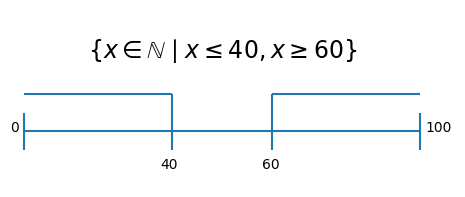
\includegraphics[width=70mm]{Graphics/output.png}
    \caption{Ejemplo básico de dominio segmentado}
    \label{fig:segmentado}
\end{figure}
\newpage
\begin{listing}[!ht]
    \begin{minted}{Python}
        Domain[int] | (lambda x: (x <= 40) | (x >= 60))
    \end{minted}
    \caption{Descripción del DSL para el dominio segmentado \ref{fig:segmentado}}
    \label{lst:segmentado}
\end{listing}

El primero de estos dos dominios, es el dominio segmentado. Este es el resultado de la operación lógica ``{\bf o}'' entre dos
restricciones distintas, como muestra el ejemplos \ref{lst:segmentado}. 
Dicha operación representa la unión de dos dominios, véase el figura \ref{fig:segmentado}, los cuales 
en principio pudieran ser infinitos, la representación elegida fue la de una clase nueva que referencié a ambos dominios y 
que en el momento de la generación la misma escoja entre uno de ellos de forma aleatoria para que este genere el resultado final.

La última clase de la jerarquía de dominios representa a las transformaciones lineales de un espacio a otro. 
La cual fue implementada para resolver las restricciones modulares. Estas restricciones transforman los espacios 
numéricos en una lista infinita de opciones. Pero analizando el dominio siguiente. 

\begin{align*}\label{modular}
    A := \Set{x \in \mathbb{Z}}{ x \equiv 1 (mod\ 2), 0 \leq x \leq 10} \\ 
\end{align*}
Se puede inferir que:
\begin{equation} \label{eq1}
    \begin{split}
    & \Rightarrow x = 2 * \alpha + 1, x \in [0, 10] \\
    & \Rightarrow \alpha = (x - 1)/2, \alpha \in [0, 4] \\ 
  \end{split}
\end{equation}

Realizado un análisis similar se implementó dicha última clase de la jerarquía de dominios. 
La misma, al igual que la clase implementada para los dominios segmentados, contiene uno de los dominios básicos en su interior,
aunque en este caso este dominio únicamente puede ser numérico, como se muestra en el ejemplo \ref{lst:tranformation}. 
Con esta idea la biblioteca puede analizar también aquellas restricciones que no son escritas de forma tal que el parámetro 
que hace referencia a un elemento cualquiera del espacio en cuestión quedase despejada, por ejemplo $x + 10 < 0$ en vez de $x < -10$. 

\begin{listing}[!ht]
    \begin{minted}{Python}
    Domain[int](-10, 100) | (lambda x: (x % 2 == 1, 0 <= x, x <= 10))
  
    # Al detectar la restricción modular, 
    # el dominio de enteros inicial 
    # se transforma a:
    # 
    # LinearTransformedDomain(
    #   original_domain=N(-10, 100), 
    #   transformer=lambda x: x/2,   
    #   inverse=lambda x: x * 2,         
    #   independent_value=1
    # )
    \end{minted}
    \caption{Transformaciones lineales de los dominios}
    \label{lst:tranformation}
\end{listing}

Cada uno de los espacios de búsqueda definidos inicialmente por la biblioteca determinan explícitamente su tipo de dominio
inicial y los distintos recorridos por los {\bf ASTs} que dicha clase necesita para inferir los límites reales y dinámicos
descritos por el usuario. Todos los procesos y análisis realizados a partir de la información contenida en los ASTs de
restricciones fueron implementados siguiendo el patrón de diseño visitante (Visitor Design Pattern, (\cite{vistorpattern})). El resultado final
cuenta con 7 de estos recorridos los cuales son creados o inyectados en los distintos espacios de búsqueda en dependencia
de la función que cumpla dicho espacio en la jerarquía descrita por el usuario.

El más importante de los recorridos implementados es aquel que modifica los dominios de los espacios de búsqueda de los
tipos básicos. Como se comentó anteriormente y se detallará más adelante, todas las restricciones descritas por el usuario
se trasladan hacia las hojas de la jerarquía descrita donde se encuentran los tipos básicos. Una vez que cada uno de los
tipos básicos contienen en su {\bf AST} todas aquellas restricciones que los referencian, se analiza cada árbol de dichos {\bf ASTs}
para clasificarlos en las categorías antes descritas. En los casos en los que dicho árbol no contenga restricciones
contextuales se realiza un recorrido sobre el mismo para modificar el dominio inicial del espacio.

El recorrido de modificación de dominio no es más que un {\bf DFS} por el {\bf AST}. Una vez se resuelven los valores específicos de cada
hoja del árbol, se le aplica al dominio en cuestión cada una de las operaciones descritas en el interior de {\bf AST}. Cada una de
las clases de la jerarquía de dominios cuenta con la implementación de todos los operadores que pueda soportar el mismo, como
regla generar dicha implementación retorna un nuevo dominio modificado. Al finalizar este recorrido, el dominio dinámico
resultante es el más grande subconjunto del dominio inicial, tal que la mayoría los valores en su interior cumplen con las
restricciones descritas.

Nótese que en dicho subconjunto la mayoría cumplen con las restricciones, y es que como se ha mencionado anteriormente existen
casos en los que la biblioteca únicamente puede resolver los problemas a partir de la filosofía “prueba y error”. En la 
tabla \ref{chap2:examples} se ejemplifican algunos de los casos más ilustrativos del mecanismo de modificación de dominios, además el primero de dichos
ejemplos es uno de los casos más sencillos donde la herramienta se ve obligada a dejar elementos no factible en el interior del
dominio.

\setlength\LTleft{-3cm}
\setlength\LTright{-5cm}
\begin{longtable}{ | p{6cm} | p{2cm}| p{3.5cm}| p{6.5cm}|  }
    \caption{Ejemplos de la restricción de distrintos dominios y sus resultados }\label{chap2:examples} \\
    \endfirsthead
    % \multicolumn{1}{c}{\tablename\ \thetable\ -- \textit{Continued from previous page}} \\
    \hline
    \endhead
    \hline
    % \multicolumn{1}{r}{\tablename\ \thetable\ -- \textit{Continued on next page}}       \\
    \endfoot
    \hline
    \endlastfoot

    % --------------------------------------------------------------------------------------------------------------
    \textbf{Primer Operando}          &
    \textbf{Operador}                 &
    \textbf{Segundo\newline Operando} &
    \textbf{Resultado}                                                                                  \\
    % --------------------------------------------------------------------------------------------------------------
    \hline
    % --------------------------------------------------------------------------------------------------------------
    ContinuosDomain(-oo, oo)          &
    <                                 &
    5                                 &
    ContinuosDomain(-oo, 5)                                                                             \\
    % --------------------------------------------------------------------------------------------------------------
    \hline
    % --------------------------------------------------------------------------------------------------------------
    NaturalDomain(-oo, oo)            &
    <                                 &
    5                                 &
    NaturalDomain(-oo, 4)                                                                               \\
    % --------------------------------------------------------------------------------------------------------------
    \hline
    % --------------------------------------------------------------------------------------------------------------
    FiniteDomain([1,...,10])          &
    <                                 &
    5                                 &
    FiniteDomain([1,...,4])                                                                             \\
    % --------------------------------------------------------------------------------------------------------------
    \hline
    % --------------------------------------------------------------------------------------------------------------
    ContinuosDomain(-oo, oo)          &
    !=                                &
    5                                 &
    ContinuosDomain(-oo, oo)                                                                            \\
    % --------------------------------------------------------------------------------------------------------------
    \hline
    % --------------------------------------------------------------------------------------------------------------
    FiniteDomain([1,...,10])          &
    !=                                &
    5                                 &
    FiniteDomain([1,...,4,6, ...10])                                                                    \\
    % --------------------------------------------------------------------------------------------------------------
    \hline
    % --------------------------------------------------------------------------------------------------------------
    NaturalDomain(-oo, oo)            &
    !=                                &
    5                                 &
    SegmentationDomain(\newline
    ... NaturalDomain(-oo, 4),\newline
    ... NaturalDomain(6, oo))                                                                           \\
    % --------------------------------------------------------------------------------------------------------------
    \hline
    % --------------------------------------------------------------------------------------------------------------
    SegmentationDomain(\newline
    ... NaturalDomain(-oo, 4), \newline
    ... NaturalDomain(6, oo))         &
    !=                                &
    10                                &
    SegmentationDomain(\newline
    ... NaturalDomain(-oo, 4),\newline
    ... NaturalDomain(6, 9), \newline
    ... NaturalDomain(11, oo) )                                                                         \\
    % --------------------------------------------------------------------------------------------------------------
    \hline
    % --------------------------------------------------------------------------------------------------------------
    NaturalDomain(0, 15)              &
    |                                 &
    FiniteDomain(\newline
    ... [20, 100,200])                &
    SegmentationDomain(\newline
    ... NaturalDomain(0, 15), \newline
    ... FiniteDomain([20, 100,200]))                                                                    \\
    % --------------------------------------------------------------------------------------------------------------
    \hline
    % --------------------------------------------------------------------------------------------------------------
    NaturalDomain(0, 15)              &
    +                                 &
    5                                 &
    LinealTransformationDomain(\newline
    ... NaturalDomain(5, 20), \newline
    ... tranformer = lambda x: x + 5, \newline
    ... inverter = lambda x: x - 5 )                                                                    \\
    % --------------------------------------------------------------------------------------------------------------
    \hline
    % --------------------------------------------------------------------------------------------------------------
    LinealTransformationDomain(\newline
    ... NaturalDomain(5, 20),\newline
    ... tranformer = lambda x: x + 5,\newline
    ... inverter = lambda x: x - 5)   &
    <                                 &
    10                                &
    LinealTransformationDomain(\newline
    ... NaturalDomain(5, 15),\newline
    ... tranformer = lambda x: x + 5,\newline
    ... inverter = lambda x: x - 5 )                                                                    \\
    % --------------------------------------------------------------------------------------------------------------
    \hline
    LinealTransformationDomain(\newline
    ... NaturalDomain(5, 20),\newline
    ... tranformer = lambda x: x + 5, \newline
    ... inverter = lambda x: x - 5)   &
    !=                                &
    10                                &
    LinealTransformationDomain(\newline
    ... SegmentationDomain(\newline
    ...... NaturalDomain(5, 14), \newline
    ...... NaturalDomain(16, 20)), \newline
    ... tranformer = lambda x: x + 5,\newline
    ... inverter = lambda x: x - 5)                                                                     \\
    % --------------------------------------------------------------------------------------------------------------
    \hline
\end{longtable}

En dicho primer ejemplo se tiene un espacio de búsqueda de números reales, por lo tanto su dominio inicial es un dominio decimal acotado.
Todos los dominios numéricos acotados se modelan mediante clases de {\bf Python} con las propiedades {\bf min} y {\bf max}. 
En dicho ejemplo el usuario describe que todo elemento perteneciente
al espacio es menor estricto que 5. Dicha restricción es resuelta con el recorrido antes explicado, realizando la misma operación sobre
el dominio en cuestión. Nótese que para que dicho dominio cumpla con esta restricción únicamente necesita comparar su límite superior
con el valor especificado, y en caso de que dicho límite sea superior cambiarlo. Si el espacio de búsqueda fuera de números naturales y
límite superior fuera mayor que 5, como es el caso del segundo ejemplo de la tabla anterior, entonces el nuevo límite sería 4, dejando
el subconjunto más grande donde todos cumplen con la restricción. Sin embargo, al ser un dominio decimal resulta más conveniente
incluir un valor erróneo en el dominio, que determinar cuál es el valor que antecede a un número determinado en la aritmética del
sistema y el lenguaje.

\subsection{Reducción e Inferencia de Dominios}

Otro de los procesos importantes que se realizan en tiempo de compilación, al que ya anteriormente se le ha hecho referencia,
es la transferencia de restricciones a través de la jerarquía descrita por el usuario. Este proceso es exclusivo de los espacios
complejos como las listas y las clases. Además este es el objetivo principal de tres de los siete recorridos implementados.

Las clases y las listas en principio se pueden considerar ambos contenedores de espacios de búsquedas. Aunque existe una diferencia
principal entre estas estructuras, los espacios internos de las clases ya han sido creados incluso antes que el espacio de la clase
en cuestión, a excepción de los espacios de tipo {\bf Self}. Dichas instancias se encuentran almacenadas en los valores por defecto de
las funciones de dicha clase o como atributo estático de la misma. Mientras que, por otro lado, la clase \newline {\bf TensorSearchSpace} es la
encargada de crear cada uno de los espacios de búsquedas para cada uno de sus índices, siendo este uno de los procesos más costosos
en el interior del {\bf DSL}.

Como el espacio de las listas que se puede representar con la propuesta de solución incluye a los tensores
multidimensionales entonces la iteración por los distintos índices de una estructura cualquiera del espacio de las listas no es un
simple recorrido sino que antes de analizar cada elemento del mismo es necesario construir y detectar cada índice en el interior
de las dimensiones concretas de cada caso.

Debido a dichas diferencias el proceso de transferencia de restricciones en cada una de estas estructuras se maneja de formas
distintas. El mecanismo general para la transferencia de restricciones es que las estructuras de orden superior inyecten las
instancias de los ``visitantes'' necesarios a sus espacios internos para que estos sepan interpretar debidamente algunas operaciones
como la indexación o la referencia a atributos. Dicha inyección en el caso de las clases tiene lugar en el método \newline
{\it \_\_init\_\_} de la clase {\bf SpaceFactory}, clase encargada de manejar a todos los espacios descrito por clases del usuario. Al crear una nueva instancia
de un espacio personalizado por el usuario se filtran todos los miembros estáticos de dicha clase en búsqueda de aquellos que sean
herederos de la clase {\bf BasicSearchSpace}, se almacenan sus referencias en dicha nueva instancia y se les inyecta las herramientas
necesarias. Por otro lado, en el caso de los tensores las inyecciones ocurren cada vez que dicho espacio crea un nuevo espacio
interno para un nuevo índice. Como las dimensiones de estos tensores pueden ser fijas o dinámicas, tanto en tiempo de compilación
como en tiempo de generación puede ser necesario crear un nuevo espacio e inyectarle las herramientas necesarias.

Nótese que el hecho de que las restricciones sean traspasadas de padres a hijos a lo largo de las jerarquías descritas, implica que
cada una de las hojas conocen al detalle su posición en la jerarquía y solo dependen de sus padres para obtener las distintas
herramientas interpretativas. Debido a lo anterior se podría resumir que, todo espacio perteneciente a un tensor conoce cual es
su índice y todo espacio perteneciente a una clase conoce a que miembro él hace referencia. Partiendo de esta base, las herramientas
interpretativas antes mencionadas solo tienen la tarea de detectar cuando una operación de indexación o referencia a atributo se refiere
al espacio en cuestión o cuando es una referencia contextual a otro espacio de la jerarquía.

Para realizar dichas interpretaciones sobre el {\bf AST} de restricciones la biblioteca utiliza tres de los siete recorridos antes mencionados,
uno para los índices, otro para los miembros y un tercero para ratificar que el resultado de los dos anteriores es un {\bf AST} coherente y sin
redundancias. La interpretación de las referencias a atributos es de los dos el caso más sencillo, pues basta que la instancia de la
clase que implementa el recorrido memorice el nombre de la propiedad en cuestión y analice los nodos {\bf GetAttr} del {\bf AST} en cuestión
para transformar dichos nodos en nodos {\bf Self} o en nodos de dependencias contextuales.

Por otro lado, la interpretación de las operaciones de indexación son un tanto más complicadas debido a la flexibilidad expresiva de
la herramienta. Como ya se explicó en secciones anteriores, las variables sin valor por defecto de las funciones de restricciones a
excepción de la primera representan cada una un índice del tensor subyacente. Dichas variables soportan tanto operaciones aritméticas
como de comparación. Una operación aritmética como índices de una indexación hace referencia al resultado de dicha operación sustituyendo
el índice del elemento en cuestión. Mientras que una comparación u operación lógica hace referencia al índice en cuestión si el resultado
de la operación es verdadero, en caso contrario dichas restricciones no son tomadas en cuenta para el elemento del índice en cuestión.
Una vez resueltos los distintos valores de todas las indexaciones si los índices coinciden con la posición del espacio en cuestión dentro
del tensor entonces se remplaza dichos nodos por nodos {\bf Self} o en caso contrario por nodos de dependencias contextuales.

En las primeras ideas de solución siempre que las dependencias circulares fueran imposible de representar debido a
las reglas gramaticales y semánticas del lenguaje. Pero, todas las interpretaciones posteriores a las definiciones no solo hicieron
que se tornan muy complicada la definición de dichas reglas, sino que además dicha idea limitaba en gran
medida el potencial expresivo de la herramienta. Debido a todo lo anterior, la biblioteca cuenta con las herramientas necesarias para
soportar dependencias circulares únicamente dentro de la misma estructura. Dichas herramientas se encuentran integradas dentro de los
tres recorridos antes descritos.

Entre la lista de clases que describe a los posibles {\bf ASTs} de restricciones existe una clase especial para expresar entre otras cosas
la detección de dependencias circulares. En muchos casos las dependencias circulares internas expresadas mediante las
funciones de restricciones son simétricas, por lo que basta con solo modelar una de las dos restricciones dejando una variable libre
y otra dependiente. Una vez uno de los recorridos antes descrito detecta una dependencia circular dicho nodo se remplaza por el nodo {\bf NotEvaluate},
nodo que una vez detectado por el resto de los recorridos inválida dicho recorrido y se continúa analizando el resto de los {\bf ASTs}.
Dicho mecanismo se utiliza además en casos como la referencia a índices fuera de rango para poder modelar dependencias secuenciales
sin caer en procesos infinitos.
% “La biblioteca no hace distinción entre operaciones simétricas y no simétricas, en caso de que no sea simplemente las muestras
% generadas no pasarían la etapa de revisión de coherencia y consistencia”


Una vez determinado todos los tipos concretos de los distintos espacios de búsqueda, optimizados todos los dominios iniciales y
almacenados los {\bf ASTs} de restricciones, la biblioteca cuenta con toda la infraestructura necesaria para comenzar la explotación
de las descripciones realizadas y la generación de muestras de las mismas. Proceso que inicia en el momento que el usuario
utilice una de sus espacios descritos para llamar al método {\it get\_sample}, método que tienen como resultado la muestra generada y
el contexto en el que se desarrolló dicha generación.

\subsection{Implementación del Mecanismo Generativo}

El método {\it get\_sample} de los espacios de búsqueda espera como parámetro opcional un contexto de generación, en casos de no
obtenerlo se crea uno por defecto antes de iniciar la generación. Estos contextos son estructuras jerárquicas en las que se
almacena por niveles las muestras de cada uno de los espacios de búsqueda que fueron analizados frente al mismo. Dichos niveles
son creados por los espacios de búsqueda de orden superior para desechar muestras que no sean consistentes con restricciones
estructurales que no puedan ser trasmitidas y cumplidas por cada unidad en particular. Gracias a dichos contextos se puede
garantizar que un mismo espacio de búsqueda con un mismo contexto siempre genera la misma muestra. Además de que permite la
detección de dependencias circulares registrando todos los espacios que comienzan su proceso de muestreo.

El proceso de generación de muestras, luego de consultar al contexto en cuestión y validar que el espacio en cuestión no ha
generado ninguna muestra ni ha comenzado su generación, se divide en tres momentos principales: 1) inferencia del dominio
dinámico, 2) generación de la muestra y la validación de la misma. En la figura \ref{chap2:algo} se muestra el pseudocódigo de dicho
proceso generativo donde se puede ver que, como se ha mencionado en múltiples ocasiones, aunque se realizarón todos los
esfuerzos por evitar de la filosofía “prueba y error” esta siempre va a estar presente cuando se habla de generación de
instancias condicionales.

\begin{algorithm}[H]
    \SetAlgoLined
    \KwData{context and local domain}
    \KwResult{sample of search space and context of generation}
    \Begin{
        $domain, ast\_result \longleftarrow Domain Optimization$\;
        \While{the sample is invalid}{
            $sample \longleftarrow New Sample$\;
            ValidateSample by ast\_result

            \If{sample is invalid and type of current search space is basic}{
                domain $\longleftarrow$ domain  !=  sample;
            }
        }
        $context \longleftarrow Save Sample$\;
        \Return{(sample, context)}
    }
    \caption{Algoritmo Básico de Generando de Muestras\label{chap2:algo}}
\end{algorithm}


El primer paso de la generación de muestras, luego de las distintas consultas realizadas al contexto,
es la inferencia de los dominios dinámicos. En esta fase de la generación se realizan todos los procesos
de interpretación y reducción de dominios que se realizan en tiempo de compilación, solo que en estas
instancias únicamente se analizan aquellos {\bf ASTs} donde existan dependencias contextuales. 
En estos casos, junto al dominio actual, a los recorridos se les proporciona el contexto de generación. 
Una vez se detecta una dependencia contextual se genera una muestra para el espacio referenciado coherente con el 
contexto en cuestión. El resultado de dicho proceso sustituye al espacio referenciado en el {\bf AST} resultante 
del recorrido en cuestión. En ocasiones anteriores se resaltó que la biblioteca detectaba la estructura topológica de 
las descripciones, estructura que se encuentra plasmada en los distintos {\bf ASTs}, y que la generación de muestras 
se ordenaba en orden ascendente al número de dependencias de cada espacio. Pero, aunque lo anterior es la base 
teórica que sostuvo el desarrollo del {\bf DSL}, en la práctica ambas ideas son características implícitas en la 
filosofía recursiva de la solución.

El resultado final de esta primera etapa es un nuevo dominio dinámico, lo más ajustado posible a las restricciones
y coherente con las muestras generadas durante el proceso de inferencia, y un nuevo {\bf AST}, resultado de todas las
posibles interpretaciones realizadas al {\bf AST} inicial. En este nuevo {\bf AST} se une el resultado de los recorridos
realizados por las restricciones con dependencias contextuales, con las representaciones de aquellas otras restricciones
que no presentaban dichas dependencias, anteriormente ya se comentó que en tiempo de compilación ambos conjuntos
se almacenan en registros distintos. Este nuevo {\bf AST}, como se puede ver en el pseudocódigo anterior, será el que se
utilizará para realizar las comprobaciones finales.

Una vez realizadas todas las inferencias y reducciones posibles comienza la generación de muestras. Este paso es
la más fuerte evidencia de que los únicos procesos realmente aleatorios son la generación de números y la selección de
opciones, mientras que el resto de los mecanismos se basan en la composición de estructuras. Todos los tipos básicos
(enteros, decimales, espacios categoricales y booleanos) contienen su propia distribución aleatoria, una instancia de
la clase {\bf Sampler}. Toda instancia de dicha clase contiene un método por cada uno de estos tipos básicos y cada uno de
estos métodos, en dependencia del espacio en cuestión, espera los límites del dominio inferido o los elementos en este.
Cada uno de estos métodos generan una muestra aleatoria, según la distribución en cuestión, dentro de los límites
suministrados y coherente con el tipo solicitado. En otras palabras, el segundo paso del mecanismo generativo implementado
para los tipos básicos se reduce al uso de una de las funciones de la distribución interna del espacio en cuestión y a la
interpretación del dominio respectivo como parámetros de dichas funciones.

Por otro lado, se pueden ver otros 3 espacios que a pesar de ser especiales no presentan mayor complejidad. El primero es el
espacio vacío, desarrollado para agregar la opcionalidad a la lista de herramientas descriptivas del {\bf DSL}. Este espacio en
particular se limita a devolver el valor especial del lenguaje {\bf None}. El segundo es la clase {\bf SelfSpace}, esta clase no es
más que una ``caja'' que se crea vacía inicialmente hasta el momento en que se puede conocer el tipo real al que este espacio hace
referencia, en dicho instante se realiza una copia de dicho espacio y se coloca en el interior de esta ``caja''. 
Una vez se resuelve el tipo real de una clase {\bf SelfSpace} dicha instancia pasa a ser una simple interfaz para 
comunicar su espacio interno con el resto herramientas y operaciones.
Por último, el {\bf DSL} brinda una definición para la operación unión entre tipos distintos.
Para esto se implementó una nueva clase que a grandes rasgos es muy similar a un espacio categorical, 
salvo que al momento de generar muestras este espacio realiza dos generaciones. 
La primera generación consiste en la
selección del tipo al que pertenecerá el resultado final, y luego utilizando un espacio previamente creado y relativo a dicho tipo
se genera la muestra final. Estos tres espacios especiales son el resultado de la integración del {\bf DSL} propuesto con la biblioteca
    {\bf typing} de {\bf Python}.

Finalizando la lista de tipos de generaciones con los dos espacios que representan la parte constructiva del proceso de generación,
las clases y los tensores. Dichos espacios como ya se comentó anteriormente, aunque se encuentran dentro de la misma categoría tiene
procesos muy distintos. La generación de tensores es un proceso únicamente recursivo, iterando por cada uno de los índices, creando
el espacio en caso de ser necesario y generando muestras de estos. El espacio de clases, sin embargo, realiza un análisis utilizando
    {\bf metaprogramación} para detectar cada uno de los espacios internos y las funciones que han sido decoradas con la sintaxis descrita en
secciones anteriores. Una vez finalizada la generación de la muestra en cuestión se le asigna un nuevo atributo {\it \_\_context\_\_},
que hace referencia al contexto en el que dicha muestra se construyó. En ambos casos, antes de comenzar a generar las muestras de
cada uno de sus espacios internos, se construye un nuevo contexto hijo del contexto en cuestión para que si la muestra
final no es coherente poder eliminar del contexto cada muestra particular con facilidad.

Una vez obtenida una posible muestra final es necesario una última fase en la que se
revisará detalladamente la coherencia y compatibilidad de la muestra con todas las restricciones planteadas. Esta última fase consiste
en un último recorrido sobre el {\bf AST} resultante del proceso de inferencia de dominios dinámicos. En este se sustituyen todos los nodos
    {\bf Self} por la muestra generada y se intentan simular todas las operaciones descritas en las funciones de restricciones. En caso de que
alguna operación no puede ser realizada o que el resultado no sea el esperado, dicho recorrido lanzara un error que provocará que el
mecanismo generativo reinicie el proceso desde el segundo paso (la generación de muestras).

Para no obligar al usuario a que los nombres de las variables internas de cada una de sus clases fueran idénticas a los espacios
estáticos definidos en las mismas, este recorrido al momento de realizar la llamada a algún atributo, luego de intentarlo de forma
natural, intenta seleccionar el espacio estático en cuestión y generar una muestra con el contexto referenciado por el atributo
    {\it \_\_context\_\_}. Si el objetivo de dicha operación fuese una muestra generada por la herramienta, entonces el atributo en cuestión se
generó con el contexto referenciado por lo que la muestra generada en esta ocasión será la misma que se utilizó para crear la instancia
generada.

En el ejemplo \ref{lst:simleautoml} se puede ver lo antes mencionado. 
Nótese en este caso como dentro de la función de restricción del 
parámetro ``{\it classifier}'' de la clase {\it SemiSupervisedClassifier} 
las referencias a miembros de las subclases de la misma siempre se realiza 
utilizando el nombre de las variables estáticas de dichas subclases. 
Por ejemplo, para hacer referencias al número de categorías del clasificador 
siempre se utiliza el nombre ``{\it NCategoryDomain}'', y nunca se hace uso de los 
nombres ``{\it n_categories}'', nombre del parámetro de la función {\it \_\_init\_\_} 
relacionado con dicho número, o ``{\it n}'', nombre de la propiedad relativa a dicha 
cantidad de las instancias generadas.


\begin{listing}[!ht]
    \begin{minted}{Python}
class AbsCluster:
    NClusterDomain = Domain[int]()
    def __init__(self, n_clusters: int = NClusterDomain) -> None:
        self.n = n_clusters

class AbsClassifier:
    NCategoryDomain = Domain[int]()
    def __init__(self, n_categories: int = NCategoryDomain) -> None:
        self.n = n_categories
....

class SemiSupervisedClassifier:
    ClusterDomain = Domain[Union[KMeans, AgglomerativeClustering]]()
    def __init__(self, 
        cluster: AbsCluster = ClusterDomain,
        classifier: AbsClassifier = Domain[Union[KNN, GaussianNB]] | (
            lambda x, c=ClusterDomain: x.NCategoryDomain == c.NClusterDomain)
    ) -> None:
        self.cluster, self.classifier = cluster, classifier
    \end{minted}
    \caption{Resumen del ejemplo \ref{lst:automl}, Ejemplo de la propuesta en escenarios AutoMLs}
    \label{lst:simleautoml}
\end{listing}